\documentclass[11pt]{article}
\usepackage{amsgen,amsmath,amstext,amsbsy,amsopn,amssymb}
%\usepackage[dvips]{graphicx,color}
\usepackage{graphicx,color}
\usepackage{graphicx,color,bm}
\usepackage{epsfig}
\usepackage{enumerate}
\usepackage{float}

%\setlength{\oddsidemargin}{0.1 in} \setlength{\evensidemargin}{-0.1
%in} \setlength{\topmargin}{-0.6 in} \setlength{\textwidth}{6.5 in}
%\setlength{\textheight}{8.5 in} \setlength{\headsep}{0.75 in}
%\setlength{\parindent}{0 in} \setlength{\parskip}{0.1 in}

\textwidth 6.3in \textheight 8.8in \topmargin -0.5truein
\oddsidemargin .15truein
\parskip .1in
\renewcommand{\baselinestretch}{1.53}  % double spaced


\newcommand{\homework}[9]{
	\pagestyle{myheadings}
	\thispagestyle{plain}
	\newpage
	\setcounter{page}{1}
	\noindent
	\begin{center}
		\framebox{
			\vbox{\vspace{2mm}
				\hbox to 6.28in { {\bf Math531:~Regression - I  \hfill} }
				\vspace{6mm}
				\hbox to 6.28in { {\Large \hfill #1 (#2)  \hfill} }
				\vspace{6mm}
				\hbox to 6.28in { {\it Instructor: #3 \hfill} }
				\hbox to 6.28in { {\it Office hours: #4  \hfill #6}}
				\vspace{2mm}}
		}
	\end{center}
	\markboth{#1}{#1}
	\vspace*{4mm}
}

% ----------------------- MATH -------------------------
\def\av{\boldsymbol a}
\def\bv{\boldsymbol b}
\def\cv{\boldsymbol c}
\def\dv{\boldsymbol d}
\def\ev{\boldsymbol e}
\def\fv{\boldsymbol f}
\def\gv{\boldsymbol g}
\def\hv{\boldsymbol h}
\def\iv{\boldsymbol i}
\def\gv{\boldsymbol j}
\def\kv{\boldsymbol k}
\def\lv{\boldsymbol l}
\def\mv{\boldsymbol m}
\def\nv{\boldsymbol n}
\def\ov{\boldsymbol o}
\def\pv{\boldsymbol p}
\def\qv{\boldsymbol q}
\def\rv{\boldsymbol r}
\def\sv{\boldsymbol s}
\def\tv{\boldsymbol t}
\def\uv{\boldsymbol u}
\def\vv{\boldsymbol v}
\def\wv{\boldsymbol w}
\def\xv{\boldsymbol x}
\def\yv{\boldsymbol y}
\def\zv{\boldsymbol z}
\def\Av{\boldsymbol A}
\def\Bv{\boldsymbol B}
\def\Cv{\boldsymbol C}
\def\Dv{\boldsymbol D}
\def\Ev{\boldsymbol E}
\def\Fv{\boldsymbol F}
\def\Gv{\boldsymbol G}
\def\Hv{\boldsymbol H}
\def\Iv{\boldsymbol I}
\def\Gv{\boldsymbol J}
\def\Kv{\boldsymbol K}
\def\Lv{\boldsymbol L}
\def\Mv{\boldsymbol M}
\def\Nv{\boldsymbol N}
\def\Ov{\boldsymbol O}
\def\Pv{\boldsymbol P}
\def\Qv{\boldsymbol Q}
\def\Rv{\boldsymbol R}
\def\Sv{\boldsymbol S}
\def\Tv{\boldsymbol T}
\def\Uv{\boldsymbol U}
\def\Vv{\boldsymbol V}
\def\Wv{\boldsymbol W}
\def\Xv{\boldsymbol X}
\def\Yv{\boldsymbol Y}
\def\Zv{\boldsymbol Z}
\def\Abf{\mathbf A}
\def\Bbf{\mathbf B}
\def\Cbf{\mathbf C}
\def\Dbf{\mathbf D}
\def\Ebf{\mathbf E}
\def\Fbf{\mathbf F}
\def\Gbf{\mathbf G}
\def\Hbf{\mathbf H}
\def\Ibf{\mathbf I}
\def\Gbf{\mathbf J}
\def\Kbf{\mathbf K}
\def\Lbf{\mathbf L}
\def\Mbf{\mathbf M}
\def\Nbf{\mathbf N}
\def\Obf{\mathbf O}
\def\Pbf{\mathbf P}
\def\Qbf{\mathbf Q}
\def\Rbf{\mathbf R}
\def\Sbf{\mathbf S}
\def\Tbf{\mathbf T}
\def\Ubf{\mathbf U}
\def\Vbf{\mathbf V}
\def\Wbf{\mathbf W}
\def\Xbf{\mathbf X}
\def\Ybf{\mathbf Y}
\def\Jbf{\mathbf J}
\def\Zbf{\mathbf Z}
\def\Am{\mathrm A}
\def\Bm{\mathrm B}
\def\Cm{\mathrm C}
\def\Dm{\mathrm D}
\def\Em{\mathrm E}
\def\Fm{\mathrm F}
\def\Gm{\mathrm G}
\def\Hm{\mathrm H}
\def\Im{\mathrm I}
\def\Gm{\mathrm J}
\def\Km{\mathrm K}
\def\Lm{\mathrm L}
\def\Mm{\mathrm M}
\def\Nm{\mathrm N}
\def\Om{\mathrm O}
\def\Pm{\mathrm P}
\def\Qm{\mathrm Q}
\def\Rm{\mathrm R}
\def\Sm{\mathrm S}
\def\Tm{\mathrm T}
\def\Um{\mathrm U}
\def\mv{\mathrm V}
\def\Wm{\mathrm W}
\def\Xm{\mathrm X}
\def\Ym{\mathrm Y}
\def\Zm{\mathrm Z}
\newcommand{\Ac}{\mathcal{A}}
\newcommand{\Bc}{\mathcal{B}}
\newcommand{\Cc}{\mathcal{C}}
\newcommand{\Dc}{\mathcal{D}}
\newcommand{\Ec}{\mathcal{E}}
\newcommand{\Fc}{\mathcal{F}}
\newcommand{\Gc}{\mathcal{G}}
\newcommand{\Hc}{\mathcal{H}}
\newcommand{\Ic}{\mathcal{I}}
\newcommand{\Jc}{\mathcal{J}}
\newcommand{\Kc}{\mathcal{K}}
\newcommand{\Lc}{\mathcal{L}}
\newcommand{\Mc}{\mathcal{M}}
\newcommand{\Nc}{\mathcal{N}}
\newcommand{\Oc}{\mathcal{O}}
\newcommand{\Pc}{\mathcal{P}}
\newcommand{\Qc}{\mathcal{Q}}
\newcommand{\Rc}{\mathcal{R}}
\newcommand{\Sc}{\mathcal{S}}
\newcommand{\Tc}{\mathcal{T}}
\newcommand{\Uc}{\mathcal{U}}
\newcommand{\Vc}{\mathcal{V}}
\newcommand{\Wc}{\mathcal{W}}
\newcommand{\Xc}{\mathcal{X}}
\newcommand{\Yc}{\mathcal{Y}}
\newcommand{\Zc}{\mathcal{Z}}
\newcommand{\alphav}{\mbox{\boldmath{$\alpha$}}}
\newcommand{\betav}{\mbox{\boldmath{$\beta$}}}
\newcommand{\gammav}{\mbox{\boldmath{$\gamma$}}}
\newcommand{\deltav}{\mbox{\boldmath{$\delta$}}}
\newcommand{\epsilonv}{\mbox{\boldmath{$\epsilon$}}}
\newcommand{\zetav}{\mbox{\boldmath$\zeta$}}
\newcommand{\etav}{\mbox{\boldmath{$\eta$}}}
\newcommand{\iotav}{\mbox{\boldmath{$\iota$}}}
\newcommand{\kappav}{\mbox{\boldmath{$\kappa$}}}
\newcommand{\lambdav}{\mbox{\boldmath{$\lambda$}}}
\newcommand{\muv}{\mbox{\boldmath{$\mu$}}}
\newcommand{\nuv}{\mbox{\boldmath{$\nu$}}}
\newcommand{\xiv}{\mbox{\boldmath{$\xi$}}}
\newcommand{\omicronv}{\mbox{\boldmath{$\omicron$}}}
\newcommand{\piv}{\mbox{\boldmath{$\pi$}}}
\newcommand{\rhov}{\mbox{\boldmath{$\rho$}}}
\newcommand{\sigmav}{\mbox{\boldmath{$\sigma$}}}
\newcommand{\tauv}{\mbox{\boldmath{$\tau$}}}
\newcommand{\upsilonv}{\mbox{\boldmath{$\upsilon$}}}
\newcommand{\phiv}{\mbox{\boldmath{$\phi$}}}
\newcommand{\varphiv}{\mbox{\boldmath{$\varphi$}}}
\newcommand{\chiv}{\mbox{\boldmath{$\chi$}}}
\newcommand{\psiv}{\mbox{\boldmath{$\psi$}}}
\newcommand{\omegav}{\mbox{\boldmath{$\omega$}}}
\newcommand{\Sigmav}{\mbox{\boldmath{$\Sigma$}}}
\newcommand{\Lambdav}{\mbox{\boldmath{$\Lambda$}}}
\newcommand{\Deltav}{\mbox{\boldmath{$\Delta$}}}
\newcommand{\Omegav}{\mbox{\boldmath{$\Omega$}}}
\newcommand{\varepsilonv}{\mbox{\boldmath{$\varepsilon$}}}

\newcommand{\eps}{\varepsilon}
\newcommand{\epsv}{\mbox{\boldmath{$\varepsilon$}}}

\def\1v{\mathbf 1}
\def\0v{\mathbf 0}
\def\Id{\mathbf I} % identity matrix
\newcommand{\ind}[1]{\mathbbm{1}_{\left[ {#1} \right] }}
\newcommand{\Ind}[1]{\mathbbm{1}_{\left\{ {#1} \right\} }}
\newcommand\indep{\protect\mathpalette{\protect\independenT}{\perp}}\def\independenT#1#2{\mathrel{\rlap{$#1#2$}\mkern2mu{#1#2}}}
\newcommand{\QED}{\begin{flushright} {\bf QED} \end{flushright}}
\newcommand{\R}{\mathbb R}
\newcommand{\Real}{\mathbb R}
\newcommand{\C}{\mathbb C}
\newcommand{\E}{\mathbb E}
\newcommand{\sgn}{\mathop{\mathrm{sign}}}
\def\Pr{\mathrm P}
\def\pr{\mathrm P}
\newcommand{\Var}{\mathop{\rm Var}}
\newcommand{\var}{\mathop{\rm Var}}
\newcommand{\Cov}{\mathop{\rm Cov}}
\newcommand{\cov}{\mathop{\rm Cov}}
\newcommand{\Corr}{\mathop{\rm Corr}}
\newcommand{\ang}{\mathop{\rm Angle}}
\newcommand{\tr}{\mathop{\rm trace}}
\newcommand{\proj}{\mathop{\rm Proj}}
\newcommand{\rank}{\mathop{\rm rank}}

\newcommand{\diag}{\mathop{\rm diag}}
\newcommand{\Diag}{\mathop{\rm diag}}
\newcommand{\sk}{\vspace{0.5cm}}
\newcommand{\ds}{\displaystyle}
\newcommand{\mb}{\mbox}
\newcommand{\wh}{\widehat}
\newcommand{\argmin}{\operatornamewithlimits{argmin}}
\newcommand{\argmax}{\operatornamewithlimits{argmax}}

\newcommand{\norm}[1]{\|#1\|}
\newcommand{\abs}[1]{\left\vert#1\right\vert}
\newcommand{\set}[1]{\left\{#1\right\}}

\newcommand{\To}{\longrightarrow}

\def\equalLaw{\stackrel{\mathcal{L}}{=}}
\def\equallaw{\stackrel{\mathcal{L}}{=}}

\def\half{\frac{1}{2}}

\usepackage{caption}

\begin{document}

\begin{title}
	{\Large\bf Homework 7, MATH 455: Due Mon, 04/30/2018}
\end{title}

\author{\bf Alexander Van Roijen}

\maketitle
{\bf Instructions}:  The homework assignment editing this \LaTeX\ document.  Download the \LaTeX\ source from the class web page and study
it to learn more about \LaTeX.  Replace the text with appropriate information.  Run ``pdflatex'' on this document.

You will submit this assignment in two parts:
\begin{enumerate}
\item Print out the PDF file and bring it to class, and
\item Send an e-mail to:
\begin{center}
gang@math.binghamton.edu
\end{center}
\emph{before class} on the due date with two attachments:
\begin{itemize}
\item The \LaTeX\ source file, and
\item The generated PDF document.
\end{itemize}
\end{enumerate}
\newpage
Please complete the following:
\begin{enumerate}
\item  Finish R exercises 11.1, 11.2, 11.3, 11.4, 11.6 of the textbook. Submit your answers for {\color{red}ALL} questions.
\begin{enumerate}
	\item 11.1
	We first take a look at the PC
	\begin{verbatim}
		> hold=prcomp(seatpos[,-c(9,1,2)])
		> print(summary(hold))
		Importance of components:
		PC1     PC2     PC3     PC4     PC5     PC6
		Standard deviation     17.1573 2.89689 2.11907 1.56412 1.22502 0.46218
		Proportion of Variance  0.9453 0.02695 0.01442 0.00786 0.00482 0.00069
		Cumulative Proportion   0.9453 0.97222 0.98664 0.99450 0.99931 1.00000
	\end{verbatim}
	Looks like the first two components explain most of the variation of our data.
	Using them for our prediction we get the following.
	\begin{verbatim}
		> cmonnow = pcr(hipcenter~.-Age-Weight,data=seatpos[],ncomp=2)
		> predict(cmonnow,testhcf,ncomp=2,interval="prediction")
		, , 2 comps
		
		hipcenter
		1 -204.4636
	\end{verbatim}
	\item 11.2
	We fit a partial least squares model to the same data and examine the number of components to use.
		\begin{figure}[H]
			\centering
			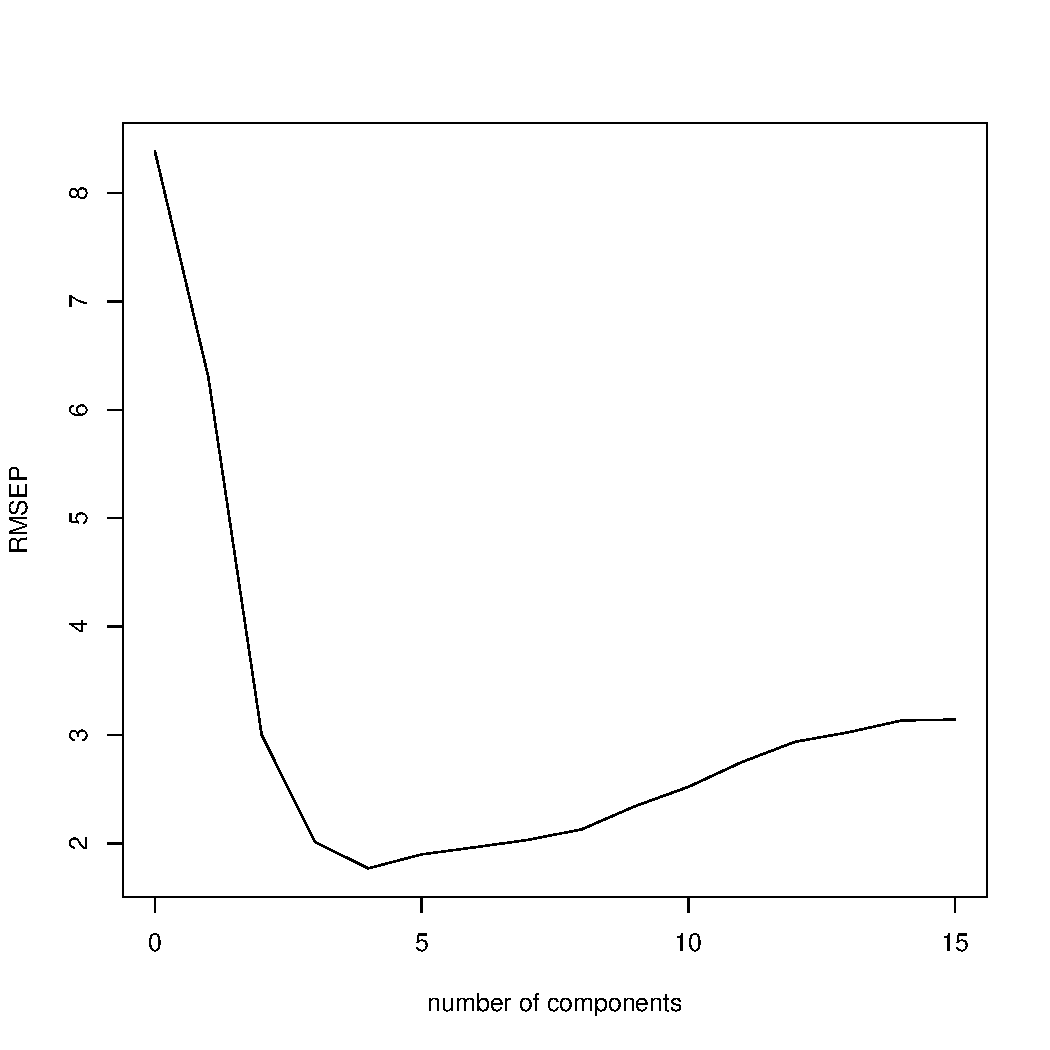
\includegraphics[width=10cm,height=10cm]{112numc.pdf}
			\caption[paic]{examining the residual mean squared error over number of components and choosing the min value}
			\label{cspos}
		\end{figure}
		we then use 4 components as it has the minmum RMSEP value and we get teh following prediction
		\begin{verbatim}
			> splsmod <- plsr(hipcenter ~ ., data=seatpos, validation="CV")
			> #4 components looks good
			> hcpred = predict(splsmod,testhcf,ncomp=4)
			> print(hcpred)
			, , 4 comps
			
			hipcenter
			1 -179.4634
		\end{verbatim}
	\item 11.3
	We are now going to fit a ridge regression model to the seatpos data
	\begin{figure}[H]
		\centering
		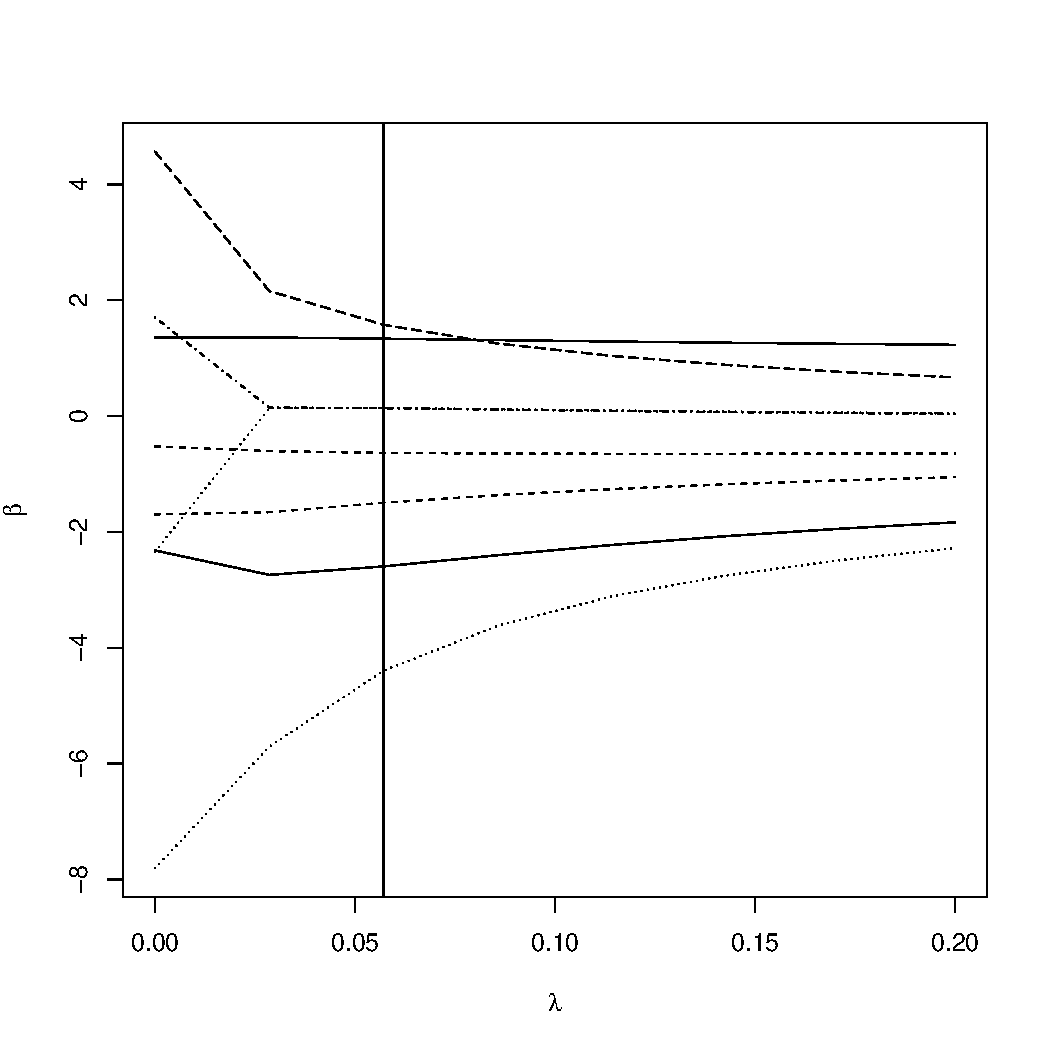
\includegraphics[width=10cm,height=10cm]{hcrgp.pdf}
		\caption[paic]{examining th}
		\label{hcrgp}
	\end{figure}
	using the minimum lambda value provided of ~0.05, we get the following prediction
	\begin{verbatim}
		> hcrgpred1 = cbind(1,as.matrix(testhcf[1,]))%*%coef(hcrgmod2)[8,]
		> hcrgpred1
		[,1]
		1 -175.488
	\end{verbatim}
	\item 11.4\\
	We first remove each tenth observation and seperate the data.
	\begin{verbatim}
		fat2=fat[-seq(1,length(fat[,1]),10),]
		testfat = fat[seq(1,length(fat[,1]),10),]
	\end{verbatim} 
	\begin{enumerate}
		\item a
		we now fit a linear model and get the following prediction accuracy described by the residual mean squared error between the predictions and the actual observations
		\begin{verbatim}
			> oglg = lm(siri ~ . -brozek -density,fat2)
			> wut=predict(oglg,newdata=testfat)
			> rmse(wut,testfat$siri)
			[1] 1.946023
		\end{verbatim}
		\item b
		we now use the stepwise function to determine the "ideal" model 
		\begin{verbatim}
			> stepwise(lm(siri ~ . -brozek -density,fat2),criterion = c("AIC"),direction=c("forward"))
			Call:
			lm(formula = siri ~ abdom + free + weight + forearm + adipos + 
			thigh + chest + biceps + ankle, data = fat2)
			
			Coefficients:
			(Intercept)        abdom         free       weight      forearm       adipos        thigh        chest       biceps  
			-2.9190       0.1179      -0.5698       0.3925       0.2146      -0.5277       0.1561       0.1246       0.1490  
			ankle  
			0.1475  
		\end{verbatim}
		I chose forward progression, and proceeded to fit a model with the chosen parameters and got the following prediction results
		\begin{verbatim}
			> splg = lm(formula = siri ~ abdom + free + weight + forearm + adipos + thigh + chest + biceps + ankle, data = fat2)
			> wut2=predict(splg,newdata=testfat)
			> rmse(wut2,testfat$siri)
			[1] 1.98911
		\end{verbatim}
		we see a slightly higher RMSE, but overall quite close and simpler too
		\item c
		Now we want to fit a principle component regression onto our data.
		\begin{verbatim}
			> print(summary(temp))
			Importance of components:
			PC1     PC2      PC3     PC4     PC5     PC6     PC7     PC8     PC9    PC10    PC11    PC12
			Standard deviation     36.8986 15.5341 10.29573 3.66009 3.44451 2.64961 2.14660 1.88702 1.57469 1.43989 1.30247 1.21438
			Proportion of Variance  0.7736  0.1371  0.06023 0.00761 0.00674 0.00399 0.00262 0.00202 0.00141 0.00118 0.00096 0.00084
			Cumulative Proportion   0.7736  0.9107  0.97095 0.97856 0.98531 0.98929 0.99191 0.99394 0.99534 0.99652 0.99749 0.99832
			PC13    PC14    PC15    PC16
			Standard deviation     1.06850 1.00511 0.75913 0.46948
			Proportion of Variance 0.00065 0.00057 0.00033 0.00013
			Cumulative Proportion  0.99897 0.99955 0.99987 1.00000
		\end{verbatim}
		I choose to only include the first 3 PRC as they cover about 97 percent of the variation in the data.\\
		Fitting the model, we now get
		\begin{verbatim}
			> fatpcr = pcr(siri ~ . -brozek -density,data=fat2,ncomp=3)
			> pcrr= predict(fatpcr,testfat,ncomp=3,interval="prediction")
			> rmse(pcrr,testfat$siri)
			[1] 2.487871
		\end{verbatim}
		the RMSE is quite higher, looking at a PCR with all PCs we get
		\begin{verbatim}
			> rmse(pcrr2,testfat$siri)
			[1] 1.946023
		\end{verbatim}
		so we could improve our RMSE, but that would effectively negate the point of PCR.
		\item d
		Looking at a partial least squares regression, we create the following
			\begin{figure}[H]
				\centering
				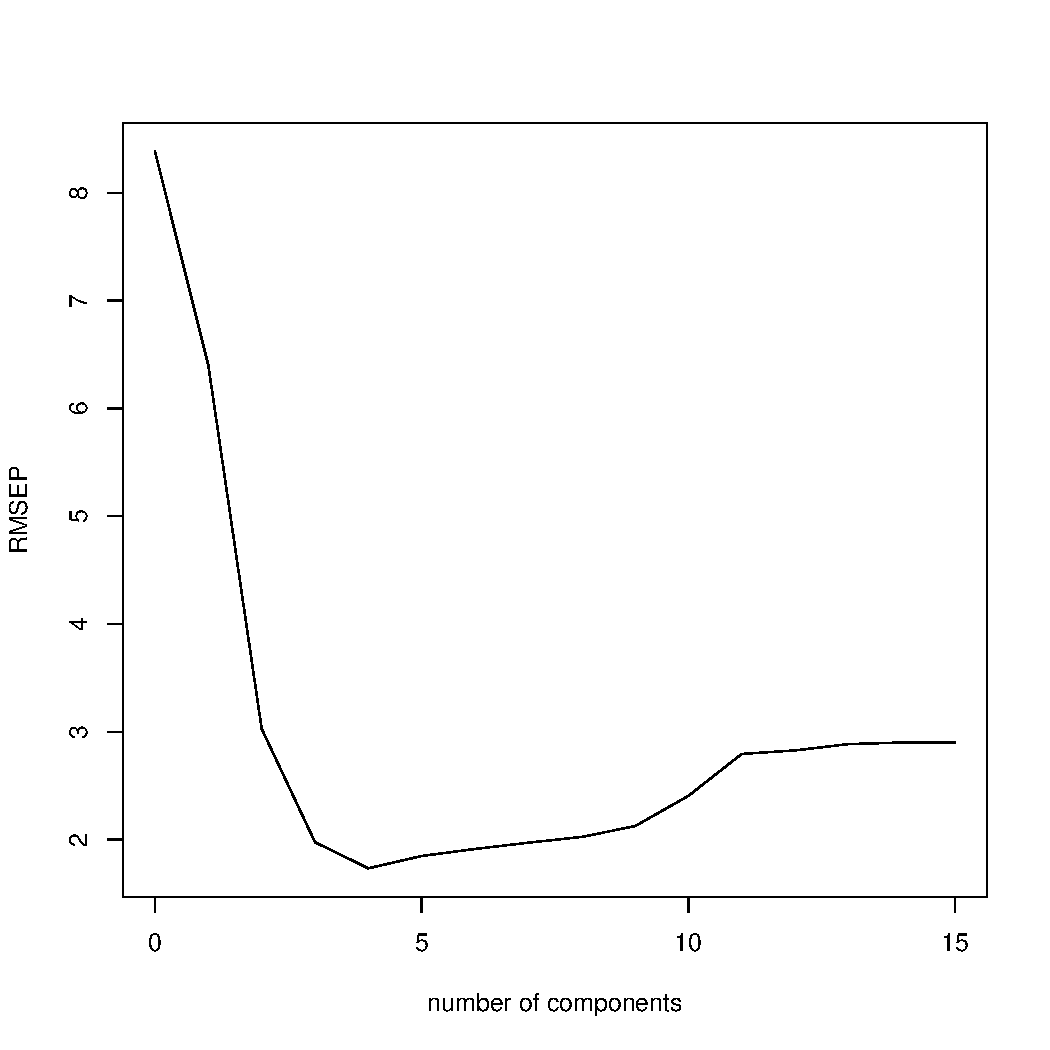
\includegraphics[width=10cm,height=10cm]{114dc.pdf}
				\caption[paic]{a look at a}
				\label{hcrgp}
			\end{figure}
		\item e
	\end{enumerate}
	\item 11.6
\end{enumerate}
\item  Finish R exercises 13.2, 13.3 of the textbook. Submit your
answers for {\color{red}ALL} questions. 
\begin{enumerate}
	\item 13.2
	\item 13.3
\end{enumerate}
\item  Finish R exercises  8.1, 8.2, 8.6, of the textbook. Submit your
answers for {\color{red}ALL} questions. 
\begin{enumerate}
	\item 8.1
	\begin{enumerate}
		\item a
		\begin{figure}[H]
			\centering
			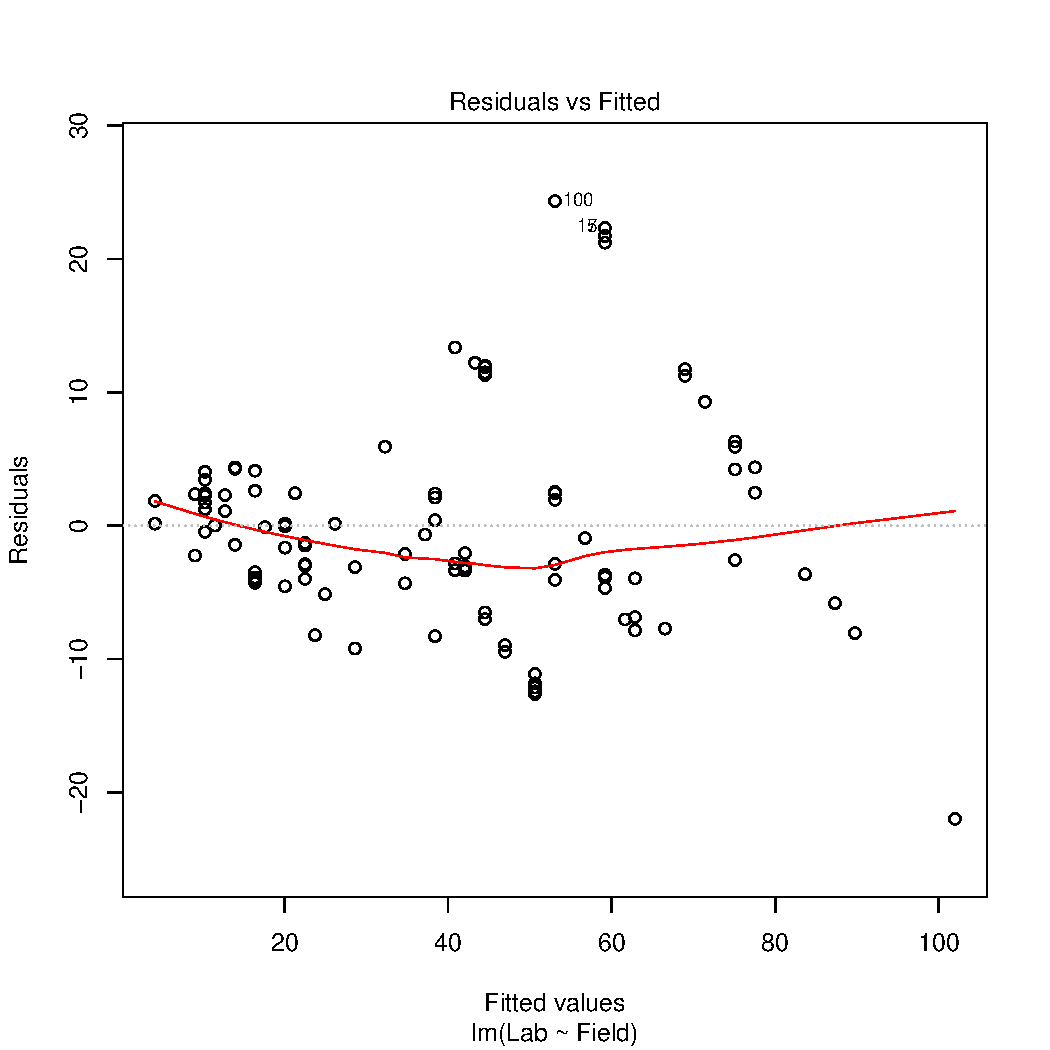
\includegraphics[width=10cm,height=10cm]{pipelinevar.pdf}
			\caption[paic]{variance check on pipeline data}
			\label{divusav}
		\end{figure}
		clearly there is some fanning here
		\item b
		\begin{verbatim}
			> summary(pipwlm)
			
			Call:
			lm(formula = Lab ~ Field, data = pipeline, weights = 1/((Field)^a_1))
			
			Weighted Residuals:
			Min      1Q  Median      3Q     Max 
			-1.7450 -0.6789 -0.2672  0.5205  2.8847 
			
			Coefficients:
			Estimate Std. Error t value Pr(>|t|)    
			(Intercept) -1.49436    0.90707  -1.647    0.102    
			Field        1.20828    0.03488  34.637   <2e-16 ***
			---
			Signif. codes:  0 ‘***’ 0.001 ‘**’ 0.01 ‘*’ 0.05 ‘.’ 0.1 ‘ ’ 1
			
			Residual standard error: 0.9795 on 105 degrees of freedom
			Multiple R-squared:  0.9195,	Adjusted R-squared:  0.9188 
			F-statistic:  1200 on 1 and 105 DF,  p-value: < 2.2e-16
		\end{verbatim}
		we see some improved R squared values as we diminish the values in order to try and prevent the fanning effect
		\item c
		\begin{figure}[H]
			\centering
			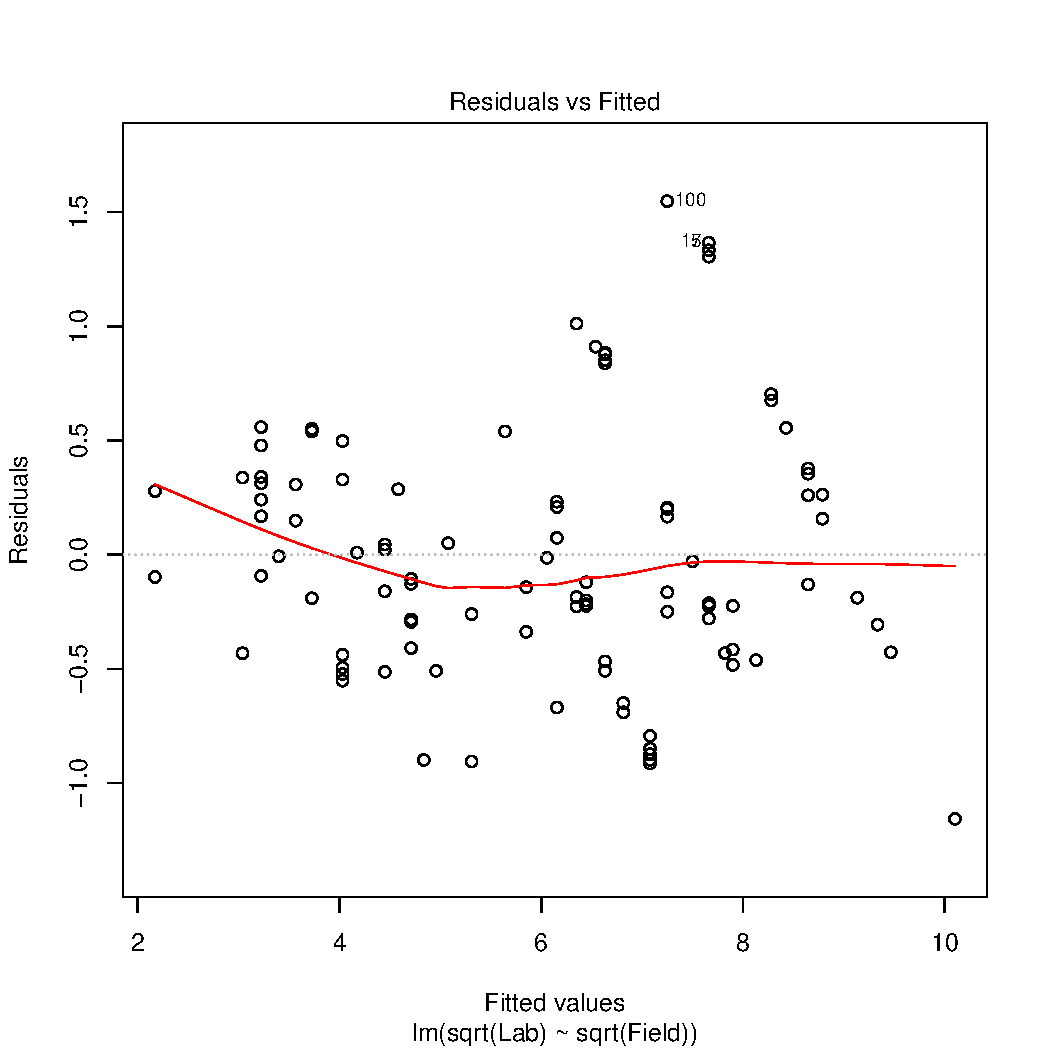
\includegraphics[width=10cm,height=10cm]{pipelinevart.pdf}
			\caption[paic]{variance check on pipeline data after transform}
			\label{divusavt}
		\end{figure}
		This is the results of taking the square root on both the response and explanatory variables. It worked quite well.
	\end{enumerate}
	\item 8.2
	\begin{enumerate}
		\item a\\
		\begin{figure}[!htb]
			\begin{minipage}{0.48\textwidth}
				\centering
				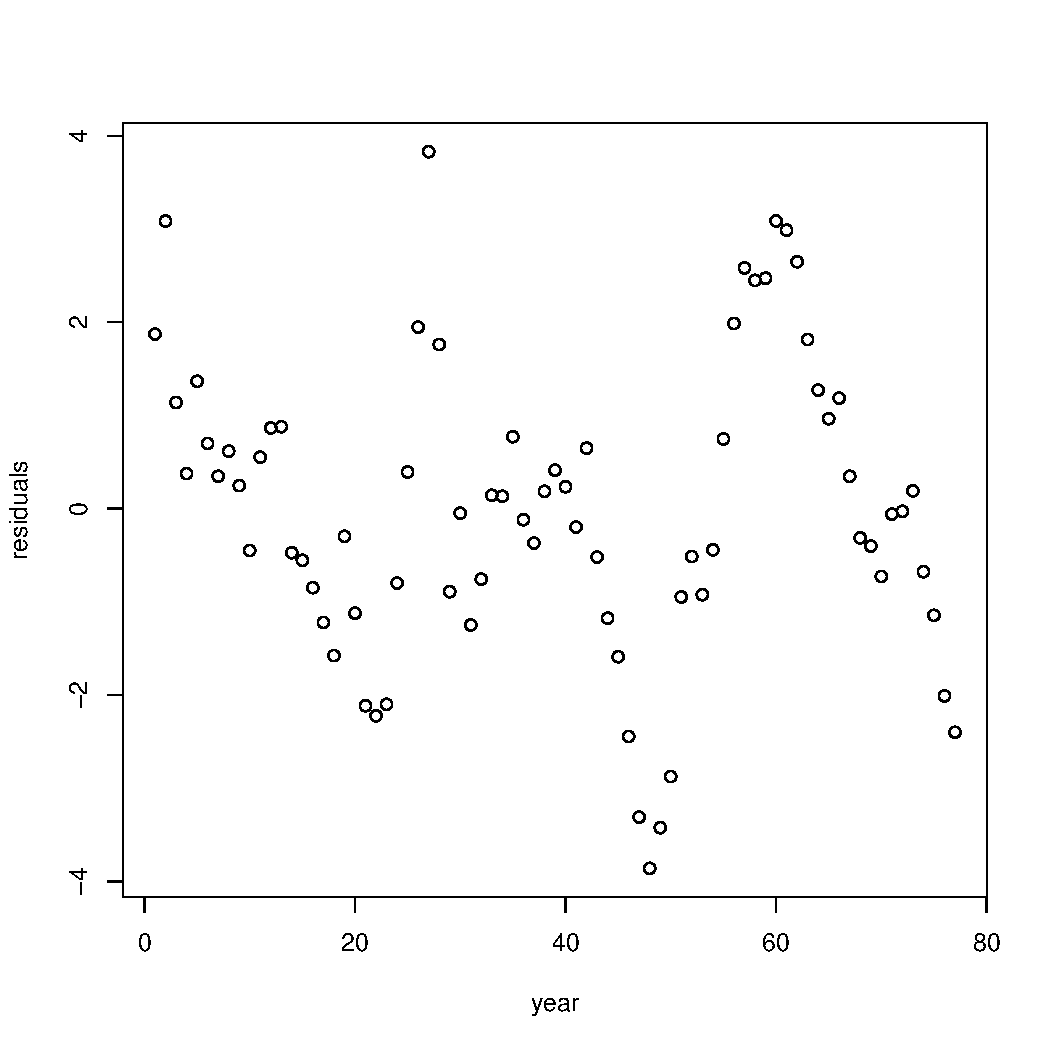
\includegraphics[width=.7\linewidth]{ovtusa.pdf}
				\caption{looking at the error correlation of divusa }\label{Fig:Data1}
			\end{minipage}
			\begin {minipage}{0.48\textwidth}
			\centering
			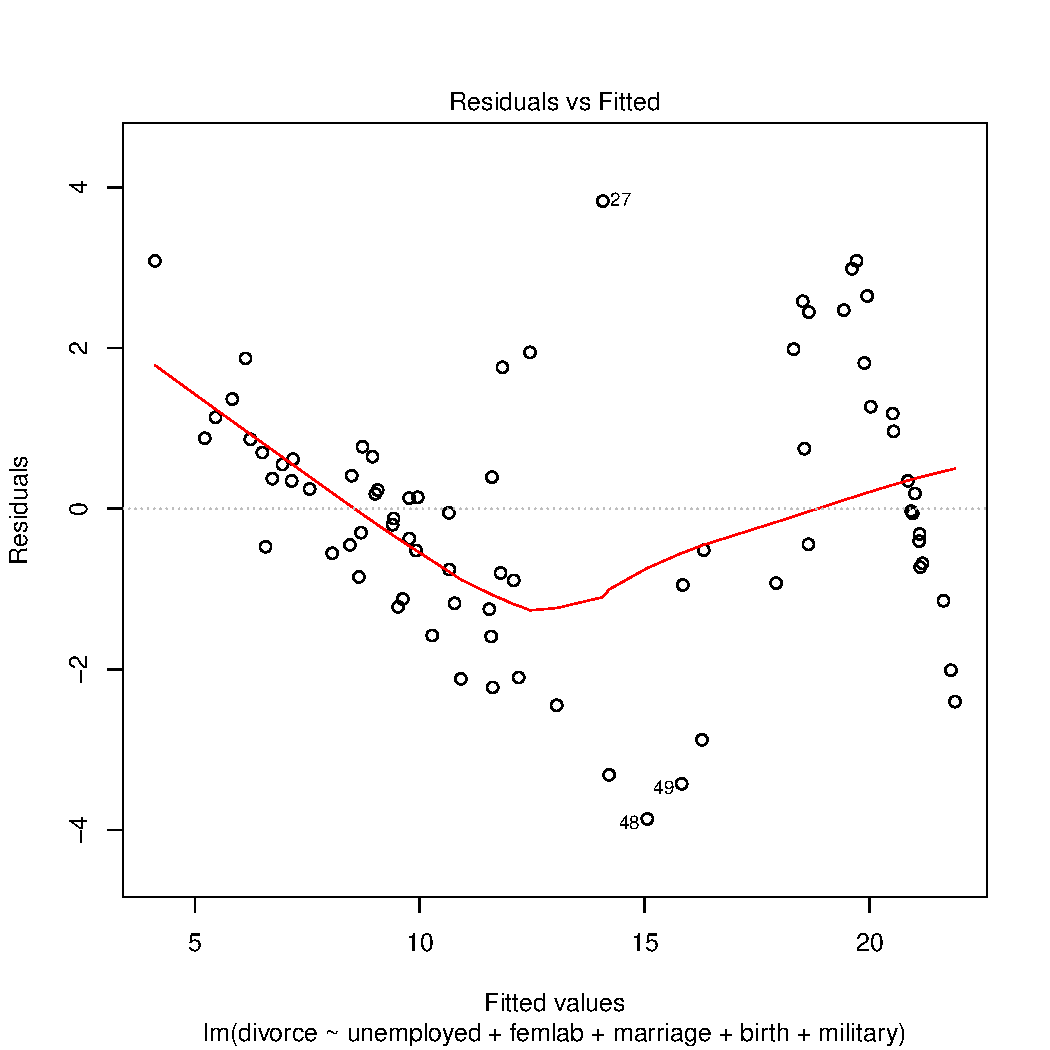
\includegraphics[width=.7\linewidth]{duse1.pdf}
			\caption{Another look at error correlation of divusa}\label{Fig:Data2}
			\end{minipage}
		\end{figure}
		we can see there is a correlation over time between the residuals/errors
		\item b
		\begin{verbatim}
			> summary(glusalm)
			Generalized least squares fit by maximum likelihood
			Model: divorce ~ unemployed + femlab + marriage + birth + military 
			Data: divusa 
			AIC      BIC    logLik
			179.9523 198.7027 -81.97613
			
			Correlation Structure: AR(1)
			Formula: ~year 
			Parameter estimate(s):
			Phi 
			0.9715486 
			
			Coefficients:
			Value Std.Error   t-value p-value
			(Intercept) -7.059682  5.547193 -1.272658  0.2073
			unemployed   0.107643  0.045915  2.344395  0.0219
			femlab       0.312085  0.095151  3.279878  0.0016
			marriage     0.164326  0.022897  7.176766  0.0000
			birth       -0.049909  0.022012 -2.267345  0.0264
			military     0.017946  0.014271  1.257544  0.2127
			
			Correlation: 
			(Intr) unmply femlab marrig birth 
			unemployed -0.420                            
			femlab     -0.802  0.240                     
			marriage   -0.516  0.607  0.307              
			birth      -0.379  0.041  0.066 -0.094       
			military   -0.036  0.436 -0.311  0.530  0.128
			
			Standardized residuals:
			Min         Q1        Med         Q3        Max 
			-1.4509327 -0.9760939 -0.6164694  1.1375377  2.1593261 
			
			Residual standard error: 2.907665 
			Degrees of freedom: 77 total; 71 residual
			> intervals(glusalm,which="var-cov")
			Approximate 95% confidence intervals
			
			Correlation structure:
			lower      est.     upper
			Phi 0.6528097 0.9715486 0.9980192
			attr(,"label")
			[1] "Correlation structure:"
			
			Residual standard error:
			lower       est.      upper 
			0.7974404  2.9076645 10.6020628 
		\end{verbatim}
		we can see that unemployed has become significant, in the previous model, the pvalue was higher.
		\\
		Further their correlation is significant, we see a positive correlation with a confidence interval that is quite strong
		\item c
		Personally, I believe these are correlated over the years mainly due to the warts the data set covers. Baby boomers are all likely to get married around the same time, and thus divorce in similar times as well. Further, War usually causes couples to get married just before leaving for service or after. Thus when they return they will realize they werent meant to be and similarly get divorced at similar times. 
	\end{enumerate}
	\item 8.6
	\begin{enumerate}
		\item a
		\begin{figure}[H]
			\centering
			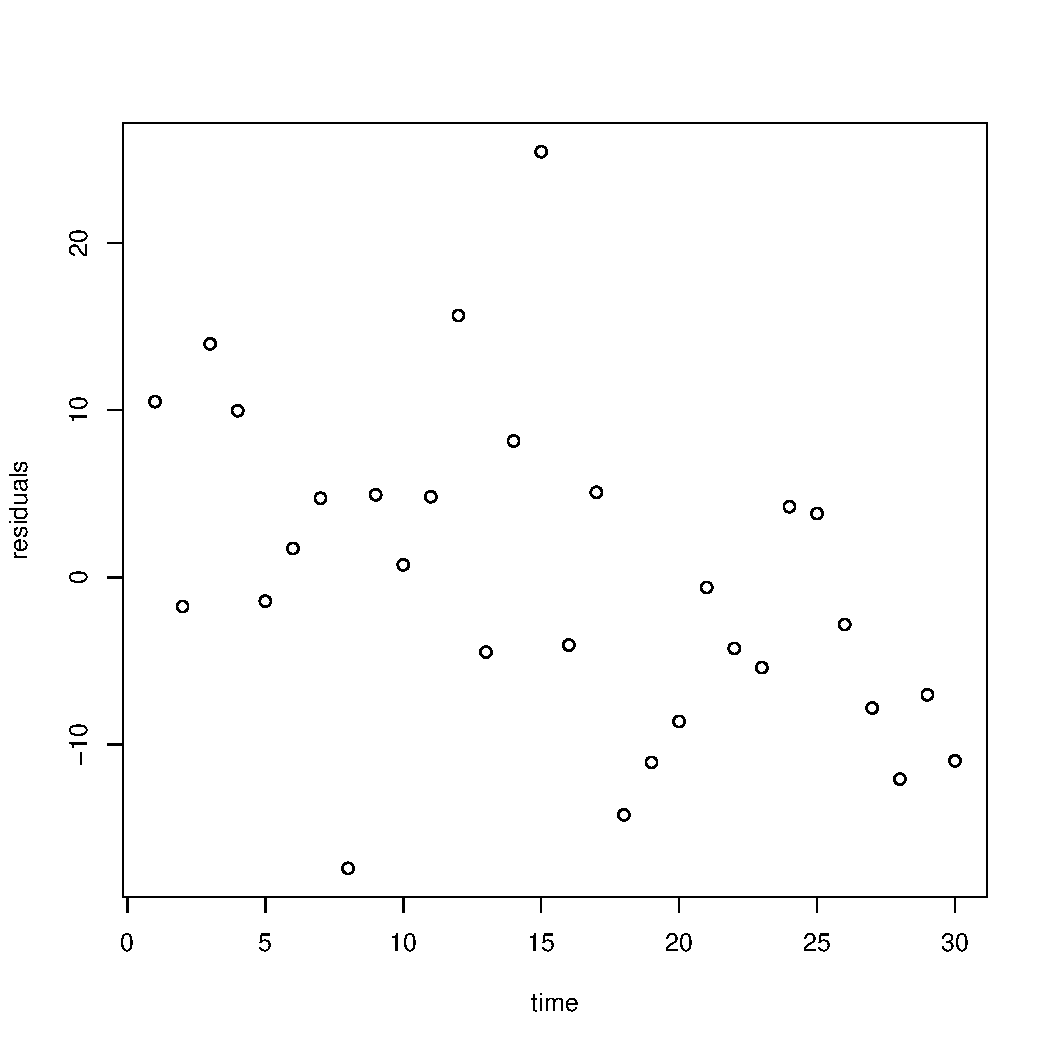
\includegraphics[width=10cm,height=10cm]{ovtc.pdf}
			\caption[paic]{we can see a somehwat linear trend over time that is decreasing.}
			\label{ovtc}
		\end{figure}
		Not a strong indicator, but something
		\item b
		\begin{verbatim}
			Generalized least squares fit by REML
			Model: taste ~ . - time 
			Data: c2 
			AIC      BIC  logLik
			214.94 222.4886 -101.47
			
			Correlation Structure: AR(1)
			Formula: ~time 
			Parameter estimate(s):
			Phi 
			0.2641944 
			
			Coefficients:
			Value Std.Error   t-value p-value
			(Intercept) -30.332472 20.273077 -1.496195  0.1466
			Acetic        1.436411  4.876581  0.294553  0.7707
			H2S           4.058880  1.314283  3.088284  0.0047
			Lactic       15.826468  9.235404  1.713674  0.0985
			
			Correlation: 
			(Intr) Acetic H2S   
			Acetic -0.899              
			H2S     0.424 -0.395       
			Lactic  0.063 -0.416 -0.435
			
			Standardized residuals:
			Min          Q1         Med          Q3         Max 
			-1.64546468 -0.63861716 -0.06641714  0.52255676  2.41323021 
			
			Residual standard error: 10.33276 
			Degrees of freedom: 30 total; 26 residual
			> intervals(cgls,which="var-cov")
			Approximate 95% confidence intervals
			
			Correlation structure:
			lower      est.     upper
			Phi -0.1690265 0.2641944 0.6118599
			attr(,"label")
			[1] "Correlation structure:"
			
			Residual standard error:
			lower     est.    upper 
			7.62646 10.33276 13.99940 
		\end{verbatim}
		We can see that the confidence interval include 0, and thus we can not really trust this correlation.
		\item 
		\begin{verbatim}
			> clm2 = lm(taste~.,c2)
			> summary(clm2)
			
			Call:
			lm(formula = taste ~ ., data = c2)
			
			Residuals:
			Min       1Q   Median       3Q      Max 
			-22.3523  -4.9735  -0.5089   4.8531  23.1311 
			
			Coefficients:
			Estimate Std. Error t value Pr(>|t|)   
			(Intercept) -36.6127    17.9845  -2.036  0.05250 . 
			Acetic        4.1275     4.2556   0.970  0.34139   
			H2S           3.5387     1.1315   3.127  0.00444 **
			Lactic       17.9527     7.7875   2.305  0.02973 * 
			time         -0.5459     0.2043  -2.672  0.01306 * 
			---
			Signif. codes:  0 ‘***’ 0.001 ‘**’ 0.01 ‘*’ 0.05 ‘.’ 0.1 ‘ ’ 1
			
			Residual standard error: 9.112 on 25 degrees of freedom
			Multiple R-squared:  0.7291,	Adjusted R-squared:  0.6858 
			F-statistic: 16.83 on 4 and 25 DF,  p-value: 8.205e-07
		\end{verbatim}
		Unlike the GLS, our OLS thinks time is significant! Very funny. However, this is not contradictory, LS and GLS are quite different. This is explained in the next part.
		\item d \\ in the GLS, we are looking at how correlated the error or noise is over "time", or consecutive entries unlike our ordinary LS. Within the OLS the time value is being included to see how it may provide information on our response. The difference lies within the relations. In OLS it changes the significance and value based on a linear combination within each entry. In residuals, we are only considering the impact of the time variable \textbf{AFTER} the coefficients have been established
		\item e\\if i was told that the entries were not in chronological order, then this would make it purely coincidental that consecutive entries are related, and we should randomize their order to avoid the seemingly correlated entries
	\end{enumerate}
\end{enumerate}
\end{enumerate}

\end{document}
